\section{Katalog Wahrscheinlichkeitsverteilungen}

\subsection[Übersicht Zufallsprozesse -- Verteilungen]{Übersicht Zufallsprozesse \textrightarrow\ Verteilungen}

\begin{center}
\begin{tikzpicture}[
  font=\footnotesize, >=Stealth,
  box/.style={draw, rounded corners=3pt, align=center, inner sep=3pt,
              minimum height=0.9cm, fill=gray!8},
  lbl/.style={font=\scriptsize\itshape, inner sep=1.5pt}]
  \node[box] (P) {Zufallsprozess\\ wählt $\omega\in\Omega$};
  \node[box, right=2.2cm of P] (X) {Zufallsvariable\\ $X(\omega)$};
  \node[box, right=2.2cm of X] (V) {Verteilung\\ $F_X(x),\ \varphi_X(x)$};
  \draw[->] (P) -- node[above, lbl] {erzeugt Wert} (X);
  \draw[->] (X) -- node[above, lbl] {hat} (V);
  \draw[->] (P.south) -- ++(0,-0.4) -| node[below, pos=0.25, lbl] {modelliert durch} (V.south);
\end{tikzpicture}
\end{center}

\begin{center}\footnotesize
\setlength{\tabcolsep}{3pt}
\renewcommand{\arraystretch}{1.75}
\begin{tabular}{l c c l}
	\textbf{Verteilung}			& $\bm{E(X)}$ 	& $\bm{\var(X)}$ 	& \textbf{Wann} \\ \hline
	Exponential ($a$)			& $\dfrac{1}{a}$ & $\dfrac{1}{a^2}$ 	& Wartezeit, gedächtnislos \\
	Erlang ($k, a$)				& $\dfrac{k}{a}$ & $\dfrac{k}{a^2}$ 	& Zeit bis $k$-tes Ereignis \\
	Poisson ($\lambda$)			& $\lambda$ 	& $\lambda$ 		& Anzahl Ereignisse in $x$ \\
	Normal ($\mu, \sigma^2$)	& $\mu$ 		& $\sigma^2$ 		& Summe vieler kleiner Einflüsse \\
	Binomial ($n, p$)			& $n p$ 		& $n p (1-p)$ 		& $n$ unabhängige Versuche \\
	Hypergeom. ($N, M, n$)		& $n \dfrac{M}{N}$ & $n p (1-p) \dfrac{N-n}{N-1}$ & ohne Zurücklegen, $p = \dfrac{M}{N}$ \\
	Gleich ($a, b$)				& $\dfrac{a+b}{2}$ & $\dfrac{(b-a)^2}{12}$ & alle Werte gleich wahrscheinlich
\end{tabular}
\end{center}

% Platz für eigene Notizen...


\subsection{Gedächtnislose Prozesse}

\subsubsection{Definition}

Die positive Zufallsvariable $T$ ist der Zeitpunkt, zu dem ein Ereignis eintritt

\vspace{0.2cm}

\begin{minipage}{0.38\columnwidth}
	$$ \boxed{ F(x) = P( T \leq x ) } $$
\end{minipage}
\hfill
\begin{minipage}{0.58\columnwidth}
	$$ \boxed{ G(x) = 1 - F(x) = P(T > x) } $$
\end{minipage}

\vspace{0.2cm}
\cgn{noch intakt nach $x$} $\Leftrightarrow T > x$ \textrightarrow\ $G(x)$
\qquad \crd{schon defekt bis $x$} $\Leftrightarrow T \leq x$ \textrightarrow\ $F(x)$


\subsubsection{Gedächtnislos}

$T$ ist gedächtnislos, wenn die Wahrscheinlichkeit, dass das Ereignis in einem Intervall eintritt, immer gleich gross ist, 
wenn es zu Beginn des Intervalls noch nicht eingetreten ist \\
\textbf{Bei gedächtnislosen Prozessen hat die Vergangenheit keinen Einfluss auf den Ausgang eines Experiments / Prozesses }

$$ \cbl{P(T \leq x+y \, | \, T > x)} = \cgn{P(T \leq y)} $$

\cgn{Wahrscheinlichkeit, dass Ereignis jetzt eintritt} \\
\cbl{Wahrscheinlichkeit, dass Ereignis später eintritt}

\vspace{0.1cm}

\textrightarrow\ \textbf{Exponentialverteilung} erfüllt diese Bedingung


\subsubsection{Beispiele für Gedächtnislose Prozesse}

\begin{tabular}{lll}
	\tabitem Etwas geht kaputt	& \tabitem Radioaktiver Zerfall	& \tabitem Warteschlangen 
\end{tabular}


\subsection{Exponentialverteilung (gedächtnislos)}

\begin{minipage}[c]{0.46\columnwidth}
	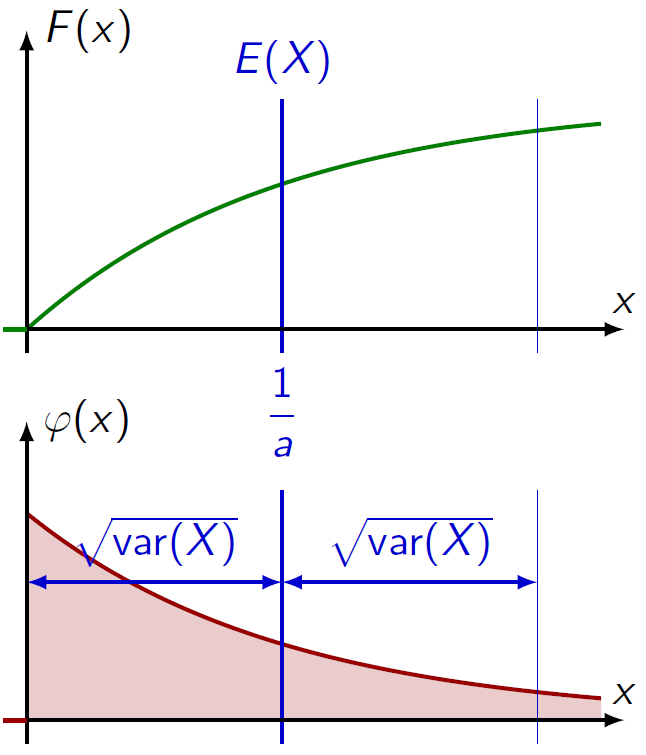
\includegraphics[width=\columnwidth]{images/exponentialverteilung.png}
\end{minipage}
\hfill
	\begin{minipage}[c]{0.52\columnwidth}
	$\cgn{F(x)} = \begin{cases} 
		0 				& x \leq 0 \\
		1 - e^{-a\, x} 	& x > 0 
	\end{cases}$

	\vspace{0.3cm}

	$\crd{\varphi(x)} = \begin{cases} 
		0 					& x \leq 0 \\
		a \, e^{-a \, x} 	& x > 0 
	\end{cases}$ 

	\vspace{0.3cm}

	Parameter: \quad $a$, $\frac{1}{a}$

	\vspace{0.2cm}

	$\frac{1}{a} = $ MTBF (Mean Time Between Failure) \\
	\textbf{( \textrightarrow\ mittlere Lebensdauer)}
\end{minipage}


\subsubsection{Eigenschaften der Exponentialverteilung}

\myul{\textbf{Erwartungswert $\bm{E(X)}$ und Varianz $\bm{\var(X)}$}}

\begin{minipage}[c]{0.3\columnwidth}
	$$ \boxed{ E(X) = \frac{1}{a} } $$
\end{minipage}
\hfill
\begin{minipage}[c]{0.66\columnwidth}
	$$ \boxed{ \var(X) = E(X^2) - E(X)^2 = \frac{1}{a^2} } $$
\end{minipage}

mit $E(X^2) = \frac{2}{a^2}$

\vspace{0.2cm}

\myul{\textbf{Lineare Näherung (kleine $a\,x$)}}
$$ F(x) = 1 - e^{-a\,x} \approx a\,x $$

\vspace{0.2cm}

\myul{\textbf{Median (Halbwertszeit) }} $\bm{t_{\frac{1}{2}}}$

\begin{minipage}[c]{0.48\columnwidth}
	$$ P(T \leq t_{\frac{1}{2}} ) = \frac{1}{2} $$
\end{minipage}
\hfill
\begin{minipage}[c]{0.48\columnwidth}
	$$ \boxed{ t_{\frac{1}{2}} = \frac{\ln(2)}{a} } $$
\end{minipage}


\vspace{0.15cm}
\textbf{Anwendungen:} Prozess ohne Erinnerungsvermögen, Radioaktivität


\subsection{Erlang-Verteilung}

\textbf{Voraussetzung:} $X_i$ ist eine \textbf{unabhängige exponentialverteilte} Zufallsvariable mit Parameter $a$

\textit{Domanda: dopo quanto \textbf{Zeit} avviene il $k$-te \textbf{Ereignis}? (\textbf{Anzahl} Ereignisse fissa, \textbf{Zeit} cercata)}


\subsubsection{Definition der Erlang-Verteilung}

\begin{minipage}[c]{0.48\columnwidth}
	$\crd{\varphi_k(x)} = \begin{cases} 
		0 											& x < 0 \\
		a^k \, \frac{x^{k-1}}{(k-1)!}\, e^{-a \, x} & x \geq 0 
	\end{cases}$ 
\end{minipage}
\hfill
\begin{minipage}[c]{0.48\columnwidth}
	$k = 1$: Exponentialverteilung
\end{minipage}


\subsubsection{Eigenschaften der Erlang-Verteilung}

\myul{\textbf{Dichte $\bm{\varphi_{k+1}(x)}$ von $\bm{T_1 + ... + T_{k+1}}$}}
$$ \boxed{ \varphi_{k+1}(x) = \varphi_k * \varphi_1 = a^{k+1} \, \frac{x^k}{k!} \, e^{-a \, x} } $$

\myul{\textbf{Summe von Erwartungswerten $\bm{E(T_1 + T_2)}$}}
$$ \boxed{ E(T_1 + T_2) = E(T_1) + E(T_2) = \frac{1}{a} + \frac{1}{a} = \frac{2}{a} } $$

\myul{\textbf{Erwartungswert und Varianz ($k$ Summanden)}}
$$ \boxed{ E(T_1 + \dots + T_k) = \frac{k}{a} } \qquad \boxed{ \var(T_1 + \dots + T_k) = \frac{k}{a^2} } $$


\vspace{0.15cm}
\textbf{Anwendungen:} Wartezeit in Telefonzentrale / am Postschalter, Warteschlangenprobleme


\subsection{Poisson-Verteilung}

\textbf{Voraussetzung:} Gedächtnislose Prozesse $T_i$ mit gleichem Parameter $a$


\subsubsection{Aufgabe}

Wie gross ist die Wahrscheinlichkeit, dass in einem Intervall der Länge $x$ genau $k$ Ereignisse / Prozesse stattfinden? \\
\textit{Domanda: quanti \textbf{Ereignisse} avvengono in un \textbf{Intervall} di lunghezza $x$? (\textbf{Zeit} fissa, \textbf{Anzahl} $k$ cercata)}
$$ P( S_k \leq x \wedge S_{k+1} > x) = F_k(x) - F_{k+1}(x) \quad \text{mit } S_k = T_1 + ... + T_k $$


\subsubsection{Poisson-Verteilung}

\begin{minipage}{0.36\columnwidth}
	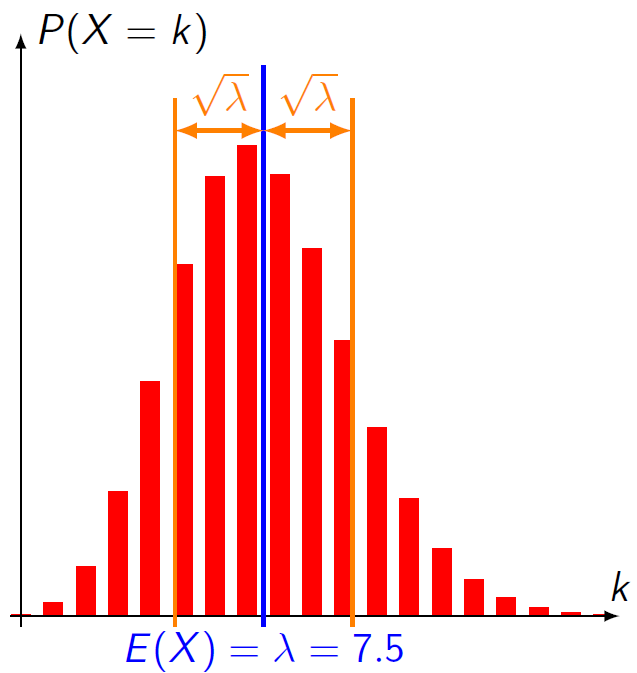
\includegraphics[width=\columnwidth]{images/poissonverteilung.png}
\end{minipage}
\hfill
\begin{minipage}{0.6\columnwidth}
	\begin{align*}
		P_k(\lambda)	&= F_k(x) - F_{k+1}(x)					\\
						&= e^{-a \, x} \frac{(a \, x )^k}{k!} 	\\
		P_k(\lambda) 	&= e^{- \lambda} \frac{\lambda^k}{k!}
	\end{align*}

	Parameter: $\lambda = a \, x$ \\
	(erwartete \# Ereignisse im Intervall $x$)
\end{minipage}

\vspace{0.2cm}

\begin{tabular}{ll}
	\cgn{$k$}		& gesuchte Anzahl Ereignisse (``genau $k$'') \\
	\cbl{$\lambda$}	& erwartete Anzahl Ereignisse im Intervall
\end{tabular}

\begin{itemize}
	\item $n$ gleiche Objekte: $\lambda = n \cdot a \cdot x$ \textrightarrow\ nicht $p = F(x)$ eines einzelnen
	\item ``weniger als $m$'' $\Rightarrow P_0 + P_1 + \dots + P_{m-1}$
\end{itemize}


\subsubsection{Eigenschaften der Poisson-Verteilung}
\label{sec:poisson-eigenschaften}

Die Poisson-Verteilung ist eine \textbf{diskrete Verteilung}

\vspace{0.2cm}

\myul{\textbf{Erwartungswert und Varianz}}
$$ \boxed{ E(X) = \var(X) = \lambda = a \cdot x } $$

\vspace{0.2cm}

\myul{\textbf{Summe von Wahrscheinlichkeiten (z.B. $\bm{P(k \leq 3)}$) }} 
$$ \boxed{ P(k \leq 3) = e^{-\lambda} \sum\limits_{k=0}^3 \frac{\lambda^k}{k!} } $$


\vspace{0.15cm}
\textbf{Anwendungen:} Anzahl Ereignisse mit exponentialverteilten Intervallen, Approximation der Binomialverteilung für seltene Ereignisse (Rate $\lambda$)


\subsection[Zufallszahlen mit Verteilung F(x)]{Zufallszahlen mit Verteilung $F(x)$}

\textbf{Voraussetzung:} $F(X)$ ist eine Verteilungsfunktion, $X$ ein im Intervall $[0,1]$ gleichverteilte Zufallsvariable


\subsubsection{Verteilungsfunktion von $Z$}

\begin{minipage}{0.25\columnwidth}
	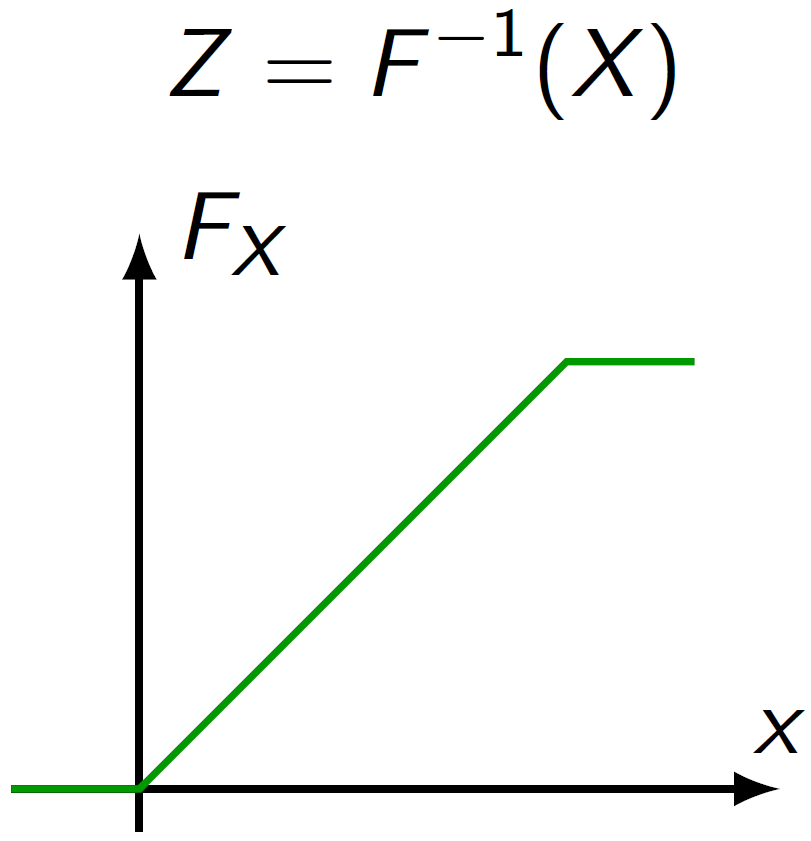
\includegraphics[width=\columnwidth]{images/verteilung_F(x).png}
\end{minipage}
\hfill
\begin{minipage}{0.7\columnwidth}
	\renewcommand{\arraystretch}{1.3}
	\begin{tabular}{r l l}
		$F_Z(z)$ 	& $= P( Z \leq z)$ 			& Definition $F_z$	\\
					& $= P(F^{-1}(X) \leq z)$ 	& Definition $Z$ 	\\
					& $= P(X \leq F(z))$ 		& Umformung 		\\
					& $= F_X(F(z))$ 			& Definition $F_X$ 	\\
					& $= F(z)$   
	\end{tabular}
	\renewcommand{\arraystretch}{1}
\end{minipage}


\subsection{Normalverteilung}

Es geht um eine \textbf{Summe vieler kleiner Einflüsse}

\vspace{0.2cm}

\begin{minipage}{0.4\columnwidth}
	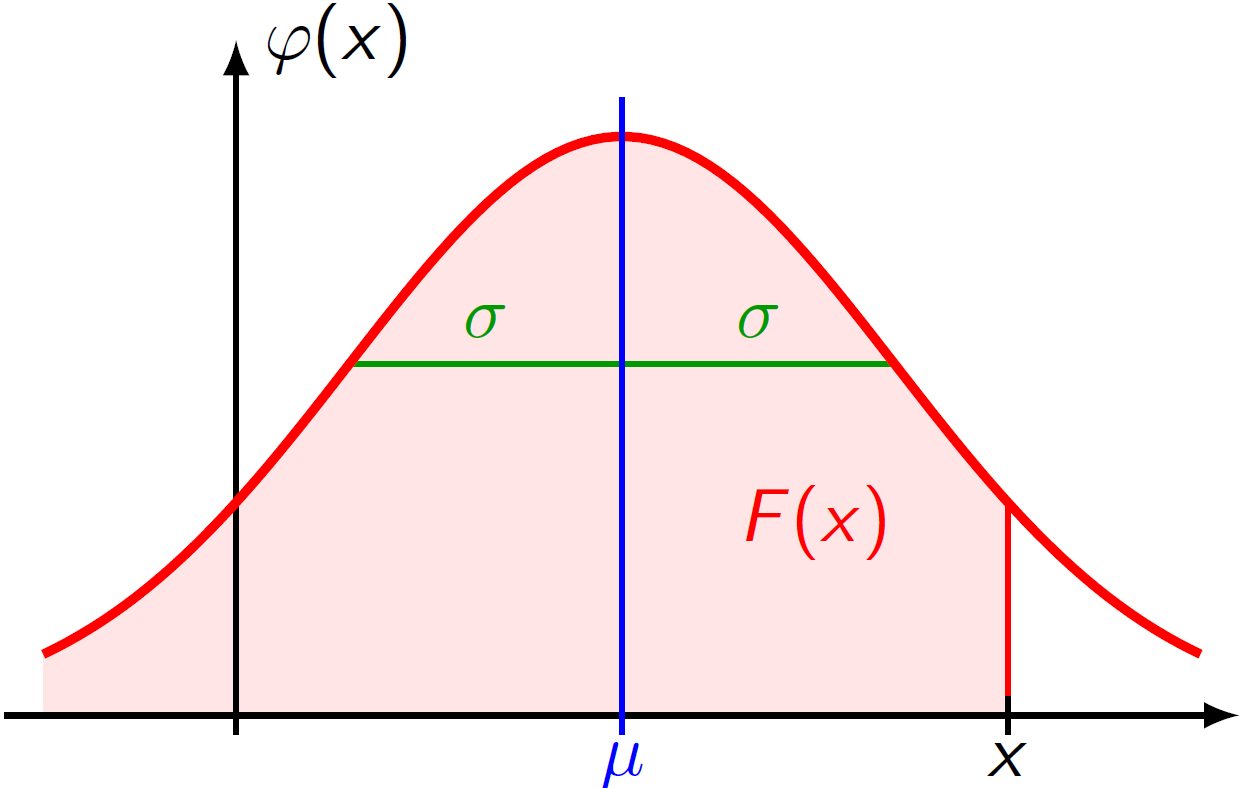
\includegraphics[width=\columnwidth]{images/normalverteilung.png}
	Maximum bei $x = \mu$ \\
	Wendepunkte bei $x = \mu \pm \sigma$ 
\end{minipage}
\hfill
\begin{minipage}{0.48\columnwidth}
	$X$ heisst \textbf{normalverteilt}, mit $E(X) = \mu$ und $\var(X) = \sigma^2$, $N(\mu, \sigma^2)$, wenn sie folgende 
	Wahrscheinlichkeitsdichte $\varphi(x)$ hat:
	$$ \boxed{ \varphi(x) = \frac{1}{\sigma \sqrt{2 \pi}} e^{- \frac{(x - \mu)^2}{2 \sigma^2}} } $$

	$\mu$ \quad Erwartungswert \\
	$\sigma$ \quad Standardabweichung 
\end{minipage}


\subsubsection{Typische Werte der Normalverteilung}

\begin{minipage}{0.45\columnwidth}
	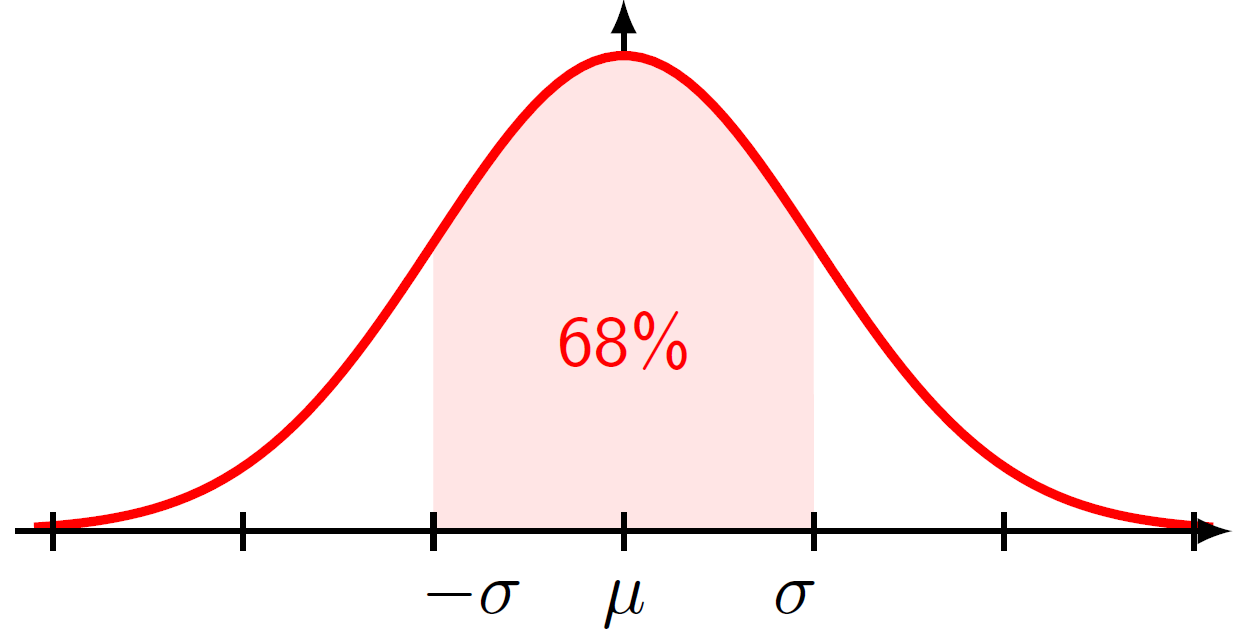
\includegraphics[width=\columnwidth]{images/normalverteilung_typische_werte.png}
\end{minipage}
\hfill
\begin{minipage}{0.45\columnwidth}
	\begin{tabular}{l c l}
		$\pm \, 1 \, \sigma$ & \textrightarrow\ & $68 \, \%$ 	\\
		$\pm \, 2 \, \sigma$ & \textrightarrow\ & $95 \, \%$ 	\\
		$\pm \, 3 \, \sigma$ & \textrightarrow\ & $99.7 \, \%$
	\end{tabular}
\end{minipage}


\subsubsection{Eigenschaften der Normalverteilung}

\myul{\textbf{Wahrscheinlichkeit}}

\vspace{0.1cm}

Wahrscheinlichkeit dafür, dass $X$ zwischen $a$ und $b$ liegt:
$$ P(a < X \leq b) = \frac{1}{\sigma \sqrt{2 \pi}} \int\limits_a^b e^{- \frac{(x - \mu)^2}{2 \sigma^2}}  \, \diff x $$


\myul{\textbf{Keine Stammfunktion}}

\vspace{0.1cm}

Die Wahrscheinlichkeitsdichte $\varphi(x)$ der Normalverteilung hat keine Stammfunktion in geschlossener Form\\ 
\textrightarrow\ Nur numerische Berechnungen möglich oder \textbf{Tabellen} verwenden

\vspace{0.2cm}

\myul{\textbf{Symmetrie}}

\vspace{0.1cm}

Die Wahrscheinlichkeitsdichte $\varphi(x)$ ist \textbf{symmetrisch} bezüglich $x = \mu$ \\
\textrightarrow\ Erwartungswert $E(X) = \mu$


\vspace{0.15cm}
\textbf{Anwendungen:} \textbf{Summe vieler kleiner Einflüsse} vergl. grosse Varianz, Messwerte, Approximation der Binomialverteilung


\subsection{Standardnormalverteilung}

\subsubsection{Standardisierung}

$X$ normalverteilt, mit $E(X) = \mu$, $\var(X) = \sigma^2$, dann ist $Z$ normalverteilt:

\vspace{0.2cm}

\begin{minipage}[t]{0.48\columnwidth}
	$$ \boxed{ Z = \frac{X - \mu}{\sigma} } $$
\end{minipage}
\hfill
\begin{minipage}[t]{0.48\columnwidth}
	\myul{\textbf{Eigenschaften}}

	\vspace{0.1cm}

	\begin{itemize}
		\item $E(Z) = 0$
		\item $\var(Z) = 1$
	\end{itemize}
\end{minipage}

% Grafica: stesso punto su due righelli (x e z)
\begin{center}
\begin{tikzpicture}[x=1.15cm, y=1.5cm, >=Stealth]
	\fill[blue!12, domain=-2.6:1, samples=50] (-2.6,0) -- plot (\x,{exp(-\x*\x/2)}) -- (1,0) -- cycle;
	\draw[thick, blue, domain=-2.6:2.6, samples=60] plot (\x,{exp(-\x*\x/2)});
	\draw[->, gray] (-2.8,0) -- (2.9,0) node[right] {\scriptsize $x$};
	\draw[->, gray] (-2.8,-0.6) -- (2.9,-0.6) node[right] {\scriptsize $z$};
	\foreach \k/\lx/\lz in {-2/\mu{-}2\sigma/-2, -1/\mu{-}\sigma/-1, 0/\mu/0, 1/\mu{+}\sigma/1, 2/\mu{+}2\sigma/2} {
		\draw[gray] (\k,0.03) -- (\k,-0.03) node[below, black, font=\tiny] {$\lx$};
		\draw[gray] (\k,-0.57) -- (\k,-0.63) node[below, orange, font=\tiny] {$\lz$};
	}
	\draw[dashed, orange] (1,-0.2) -- (1,-0.57);
	\node[blue, font=\scriptsize] at (-0.3,0.35) {$P(X \leq x)$};
	\node[orange, font=\scriptsize, anchor=west] at (1.05,-0.36) {$z = \frac{x-\mu}{\sigma}$};
\end{tikzpicture}

{\scriptsize \textbf{A colpo d'occhio:} stesso punto, stessa area -- solo un altro righello ($\sigma$ diventa 1, $\mu$ diventa 0)\par}
\end{center}


\subsubsection{Verteilungsfunktion $\Phi$  der Standardnormalverteilung}

% Grafica: Phi = area a sinistra; simmetria delle code
\begin{minipage}[t]{0.48\columnwidth}\centering
	\begin{tikzpicture}[x=0.55cm, y=1.3cm, >=Stealth]
		\fill[blue!15, domain=-3:0.8, samples=40] (-3,0) -- plot (\x,{exp(-\x*\x/2)}) -- (0.8,0) -- cycle;
		\draw[thick, blue, domain=-3:3, samples=50] plot (\x,{exp(-\x*\x/2)});
		\draw[->, gray] (-3.2,0) -- (3.3,0);
		\draw[gray] (0.8,0.04) -- (0.8,-0.04) node[below, font=\tiny, black] {$z$};
		\node[blue, font=\scriptsize] at (-0.7,0.35) {$\Phi(z)$};
	\end{tikzpicture}
	$$ \boxed{ \Phi(z) = P(Z \leq z) } $$
\end{minipage}
\hfill
\begin{minipage}[t]{0.48\columnwidth}\centering
	\begin{tikzpicture}[x=0.55cm, y=1.3cm, >=Stealth]
		\fill[orange!25, domain=-3:-1.2, samples=30] (-3,0) -- plot (\x,{exp(-\x*\x/2)}) -- (-1.2,0) -- cycle;
		\fill[orange!25, domain=1.2:3, samples=30] (1.2,0) -- plot (\x,{exp(-\x*\x/2)}) -- (3,0) -- cycle;
		\draw[thick, blue, domain=-3:3, samples=50] plot (\x,{exp(-\x*\x/2)});
		\draw[->, gray] (-3.2,0) -- (3.3,0);
		\draw[gray] (-1.2,0.04) -- (-1.2,-0.04) node[below, font=\tiny, black] {$-z$};
		\draw[gray] (1.2,0.04) -- (1.2,-0.04) node[below, font=\tiny, black] {$z$};
		\node[orange, font=\tiny] at (-2.3,0.42) {$\Phi(-z)$};
		\node[orange, font=\tiny] at (2.3,0.42) {$1-\Phi(z)$};
		\node[font=\tiny] at (0,0.42) {$=$};
	\end{tikzpicture}
	$$ \boxed{ \Phi(-z) = 1 -  \Phi(z) } $$
\end{minipage}


\example{Standardnormalverteilung}

\vspace{-0.4cm}

\begin{align*}
	P(\cbl{a} < X \leq \cor{b})	&= P \left( \frac{\cbl{a} - \mu}{\sigma} < \frac{X - \mu}{\sigma} \leq \frac{\cor{b} - \mu}{\sigma}  \right) 	\\
								&= P \left( \frac{\cbl{a} - \mu}{\sigma}  < Z \leq \frac{\cor{b} - \mu}{\sigma} \right) 						\\
								&= \Phi \Bigg( \frac{\cor{b} - \mu}{\sigma} \Bigg) -  \Phi \Bigg( \frac{\cbl{a} - \mu}{\sigma} \Bigg)
\end{align*}

\textrightarrow\ \textbf{Auswertung von $\bm{\Phi()}$ mittels Tabelle in Abschnitt \ref{Verteilungsfunktion der Normalverteilung} } \\
\textrightarrow\ \textbf{Kompakte $\bm{\Phi()}$-Tabelle in Abschnitt \ref{Quantilentabelle der Standardnormalverteilung} } 


\subsubsection{Quantilentabelle der Standardnormalverteilung / TR-Befehle}
\label{Quantilentabelle der Standardnormalverteilung}

\begin{minipage}[c]{0.4\columnwidth}

	\begin{tabular}{|l|r|}
		\hline
		$p$		&	$z = \Phi^{-1}(p)$		\\
		\hline
		0.75	&	0.6745	\\
		0.8		&	0.8416	\\
		0.9		&	1.2816	\\
		0.95	&	1.6449	\\
		0.975	&	1.9600	\\
		0.99	&	2.3263	\\
		0.995	&	2.5758	\\
		0.999	&	3.0902	\\
		0.9995	&	3.2905	\\
		\hline
	\end{tabular}
\end{minipage}
\hfill
\begin{minipage}[c]{0.57\columnwidth}
	\myul{\textbf{TI-nspire Befehle (Scratchpad)}}

	\vspace{0.2cm}

	\begin{tabular}{ll}
		$\Phi(x)$ 		& normCdf($\cbl{a}$, $\cor{b}$, $\mu$, $\sigma$)	\\
						& menu-6-5-2										\\
		\\
		$\Phi^{-1}(p)$ 	& invNorm($p$)										\\
						& menu-6-5-3
	\end{tabular}

	\vspace{0.3cm}

	\myul{\textbf{$\bm{p < 0.5}$ \textrightarrow\ $\bm{z}$ negativ}}

	\vspace{0.1cm}

	$\Phi^{-1}(p) = -\Phi^{-1}(1-p)$ \\
	z.B. $\Phi^{-1}(0.1) = -1.2816$ \\
	\phantom{z.B. }$\Phi^{-1}(0.001) = -3.0902$
\end{minipage}


\subsubsection{Rechenregeln Normalverteilung}

\myul{\textbf{Varianz $\bm{\var(X)}$}}
$$ \boxed{ \sigma^2 = \var(X) = E(X^2) - E(X)^2 } $$ 


\myul{\textbf{Summensatz $ \bm{X = X_1 + X_2}$}}

\vspace{0.1cm}
$X_1$ normalverteilt mit $E(X_1) = \mu_1$ und $\var(X_1) = \sigma_1^2$, \\
$X_2$ normalverteilt mit $E(X_2) = \mu_2$ und $\var(X_2) = \sigma_2^2$, \\
dann ist $X = X_1 + X_2$ normalverteilt mit:

\vspace{0.2cm}

\begin{minipage}[c]{0.48\columnwidth}
	$$ \boxed{ E(X) = \mu_1 + \mu_2 } $$
\end{minipage}
\hfill
\begin{minipage}[c]{0.48\columnwidth}
	$$ \boxed{ \sigma^2 = \var(X)  = \sigma_1^2 + \sigma_2^2 } $$
\end{minipage}

\vspace{0.2cm}

\myul{\textbf{$\bm{n}$ gleiche Stücke $\bm{S_n = X_1 + \ldots + X_n}$}}
$$ \boxed{ E(S_n) = n\,\mu \qquad \var(S_n) = n\,\sigma^2 \qquad \sigma_{S_n} = \sqrt{n}\,\sigma } $$

\vspace{0.2cm}

\myul{\textbf{Linearität}}

\vspace{0.1cm}

$X$ normalverteilt mit $E(X) = \mu$ und $\var(X) = \sigma^2$, dann ist $a \, X + b$ normalverteilt mit:

\vspace{0.2cm}

\begin{minipage}[c]{0.48\columnwidth}
	$$ \boxed{ E(a \, X + b) = a \, \mu +  b } $$
\end{minipage}
\hfill
\begin{minipage}[c]{0.48\columnwidth}
	$$ \boxed{ \var(a \, X + b)  = a^2 \, \sigma^2 }  $$
\end{minipage}



\subsection[Bestimmung der Parameter]{Bestimmung der Parameter $\bm{\mu}$, $\bm{\sigma^2}$}

\subsubsection{Schätzen}

\vspace{-0.2cm}

$$\hat{\mu} = E(X) = \frac{1}{n} \sum\limits_{i=1}^n x_i \text{  (Mittelwert)}$$
$$\hat{\sigma}^2 = \cor{\frac{n}{n-1}} \, (  E(X^2) - E(X)^2 ) = \cor{\frac{n}{n-1}} \, \left( \frac{1}{n} \sum\limits_{i=1}^n x_i^2 - \Big( \frac{1}{n} \sum\limits_{i=1}^n x_i  \Big)^2  \right) $$

\cor{Korrektur, damit erwartungstreu}


\subsubsection{Wahrscheinlichkeit (Standardnormalverteilung)}

$X \leq x$ mit Wahrscheinlichkeit $p$ \quad \\ {\small Text \textrightarrow\ Ereignis: \glqq höchstens $x$\grqq, \glqq bis $x$ kaputt\grqq\ $= X \leq x$ \quad \glqq hält $x$\grqq\ $= X > x$, \; $P(X \leq x) = 1 - P(X > x)$}

\vspace{0.1cm}

% Grafica: area p a sinistra di x
\begin{minipage}[c]{0.42\columnwidth}\centering
	\begin{tikzpicture}[x=0.55cm, y=1.3cm, >=Stealth]
		\fill[blue!15, domain=-3:-0.9, samples=30] (-3,0) -- plot (\x,{exp(-\x*\x/2)}) -- (-0.9,0) -- cycle;
		\draw[thick, blue, domain=-3:3, samples=50] plot (\x,{exp(-\x*\x/2)});
		\draw[->, gray] (-3.2,0) -- (3.3,0);
		\draw[gray] (-0.9,0.04) -- (-0.9,-0.04) node[below, font=\tiny, black] {$x$};
		\draw[gray, dashed] (0,0) -- (0,1) node[above, font=\tiny, black] {$\mu$};
		\node[blue, font=\scriptsize] at (-1.9,0.3) {$p$};
	\end{tikzpicture}
\end{minipage}
\hfill
\begin{minipage}[c]{0.55\columnwidth}
	$$ \Phi\Big( \frac{x - \mu}{\sigma} \Big) = p $$
	$$ \boxed{ x = \mu + \Phi^{-1}(p) \, \sigma } $$
\end{minipage}

\vspace{0.2cm}

\renewcommand{\arraystretch}{1.4}
\begin{tabular}{|l|l|l|}
	\hline
	\textbf{gegeben}			& \textbf{gesucht}		& \textbf{Weg} 											\\
	\hline
	$\mu$, $\sigma$, $x$		& $p$					& $p = \Phi\big(\frac{x-\mu}{\sigma}\big)$ (Tabelle)	\\
	$\mu$, $\sigma$, $p$		& $x$					& $x = \mu + \Phi^{-1}(p)\,\sigma$ (Quantil)			\\
	$x$, $p$ + $\mu$ o. $\sigma$	& $\sigma$ o. $\mu$	& gleiche Gleichung umstellen							\\
	\hline
\end{tabular}
\renewcommand{\arraystretch}{1}

\vspace{0.1cm}
Spezialfall Median: $p = 0.5$ \qquad  $\Phi^{-1}(0.5) = 0$ \qquad \textrightarrow\ $\mu = x$


\subsection{Zentraler Grenzwertsatz (Normalverteilung)}

Sind $X_1$, $X_2, \, \ldots$ identisch verteilte und unabhängige Zufallsvariablen mit $E(X_i) = \mu$ und \\
$\var(X_i) = \sigma^2$, dann gilt:

\renewcommand{\arraystretch}{2}
\begin{tabular}{l c l l}
	$S_n = \sum\limits_{i=1}^n X_i$ 				& \textrightarrow\	& $E(S_n) = n \, \mu$ 	& $\var(S_n) = n \, \sigma^2$	\\
	$Z_n = \frac{S_n - n \, \mu}{\sqrt{n} \sigma}$ 	& \textrightarrow\ 	& $E(Z_n) = 0$ 			& $\var(Z_n) = 1$
\end{tabular}
\renewcommand{\arraystretch}{1}

% Grafica: 1 pezzo vs somma di n pezzi (media x n, larghezza x sqrt(n))
\begin{center}
\begin{tikzpicture}[x=0.62cm, y=1.5cm, >=Stealth]
	\draw[thick, blue, domain=-1.6:1.6, samples=40] plot (\x,{exp(-\x*\x/(2*0.25))});
	\draw[thick, orange, domain=4:10, samples=50] plot (\x,{0.5*exp(-(\x-7)*(\x-7)/2)});
	\draw[->, gray] (-1.8,0) -- (10.5,0);
	\draw[gray, dashed] (0,0) -- (0,1);
	\draw[gray, dashed] (7,0) -- (7,0.5);
	\node[below, font=\tiny] at (0,0) {$\mu$};
	\node[below, font=\tiny] at (7,0) {$n\mu$};
	\draw[<->, blue] (-0.5,0.6) -- (0.5,0.6) node[right, font=\tiny] {$\sigma$};
	\draw[<->, orange] (6,0.3) -- (8,0.3) node[right, font=\tiny] {$\sqrt{n}\,\sigma$};
	\node[blue, font=\scriptsize] at (0,1.12) {1 Stück};
	\node[orange, font=\scriptsize] at (7,0.62) {Summe $S_n$};
\end{tikzpicture}

{\scriptsize \textbf{A colpo d'occhio:} media $\times n$, larghezza solo $\times\sqrt{n}$ \quad|\quad Mittelwert $\overline{X}_n = S_n/n$: \; $E = \mu$, \; $\sigma_{\overline{X}} = \sigma/\sqrt{n}$\par}
\end{center}

\vspace{0.1cm}
Für $n \to \infty$ strebt die Verteilung von $Z_n$ gegen die Standardnormalverteilung, d.h. 
$$ \lim\limits_{n \to \infty} P(Z_n \leq z) = \Phi(z) $$
\textbf{\textrightarrow\ Die Summe vieler vergleichbarer kleiner Einflüsse ist annähernd normalverteilt}

% Grafica ZGS: Summe von n gleichverteilten ZV, standardisiert, gegen N(0,1)
\begin{center}
\pgfplotsset{zgs/.style={width=1.18\linewidth, height=3.2cm, axis lines=left,
	xmin=-3.5, xmax=3.5, ymin=0, ymax=0.48, xtick={0}, ytick=\empty,
	tick label style={font=\tiny}, xlabel={$z$}, xlabel style={font=\tiny, at={(1,0)}, anchor=west},
	title style={font=\scriptsize, yshift=-1.5ex}, clip=false}}
\begin{minipage}[t]{0.32\columnwidth}\centering
	\begin{tikzpicture}
		\begin{axis}[zgs, title={$n=1$}]
			\addplot[thick, red] coordinates {(-3.5,0) (-1.732,0) (-1.732,0.2887) (1.732,0.2887) (1.732,0) (3.5,0)};
			\addplot[thin, dashed, blue, samples=60, domain=-3.5:3.5] {exp(-x^2/2)/sqrt(2*pi)};
		\end{axis}
	\end{tikzpicture}
\end{minipage}\hfill
\begin{minipage}[t]{0.32\columnwidth}\centering
	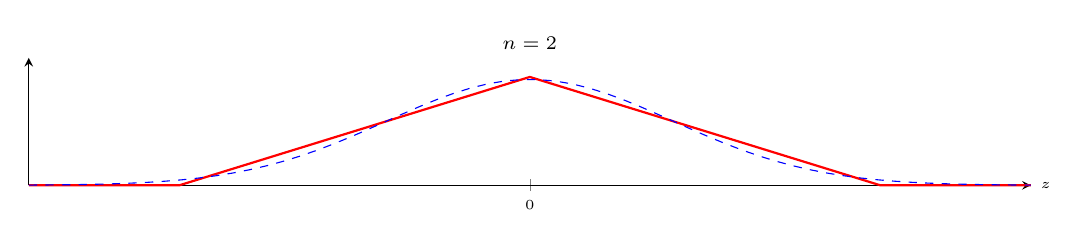
\begin{tikzpicture}
		\begin{axis}[zgs, title={$n=2$}]
			\addplot[thick, red] coordinates {(-3.5,0) (-2.449,0) (0,0.4082) (2.449,0) (3.5,0)};
			\addplot[thin, dashed, blue, samples=60, domain=-3.5:3.5] {exp(-x^2/2)/sqrt(2*pi)};
		\end{axis}
	\end{tikzpicture}
\end{minipage}\hfill
\begin{minipage}[t]{0.32\columnwidth}\centering
	\begin{tikzpicture}
		\begin{axis}[zgs, title={$n=12$}]
			\addplot[thick, red, smooth] coordinates {(-3.500,0.0006) (-3.375,0.0010) (-3.250,0.0016) (-3.125,0.0025) (-3.000,0.0038) (-2.875,0.0058) (-2.750,0.0085) (-2.625,0.0122) (-2.500,0.0172) (-2.375,0.0237) (-2.250,0.0320) (-2.125,0.0424) (-2.000,0.0552) (-1.875,0.0705) (-1.750,0.0886) (-1.625,0.1093) (-1.500,0.1326) (-1.375,0.1582) (-1.250,0.1857) (-1.125,0.2145) (-1.000,0.2440) (-0.875,0.2731) (-0.750,0.3011) (-0.625,0.3270) (-0.500,0.3497) (-0.375,0.3684) (-0.250,0.3824) (-0.125,0.3910) (0.000,0.3939) (0.125,0.3910) (0.250,0.3824) (0.375,0.3684) (0.500,0.3497) (0.625,0.3270) (0.750,0.3011) (0.875,0.2731) (1.000,0.2440) (1.125,0.2145) (1.250,0.1857) (1.375,0.1582) (1.500,0.1326) (1.625,0.1093) (1.750,0.0886) (1.875,0.0705) (2.000,0.0552) (2.125,0.0424) (2.250,0.0320) (2.375,0.0237) (2.500,0.0172) (2.625,0.0122) (2.750,0.0085) (2.875,0.0058) (3.000,0.0038) (3.125,0.0025) (3.250,0.0016) (3.375,0.0010) (3.500,0.0006)};
			\addplot[thin, dashed, blue, samples=60, domain=-3.5:3.5] {exp(-x^2/2)/sqrt(2*pi)};
		\end{axis}
	\end{tikzpicture}
\end{minipage}

\vspace{0.1cm}
{\scriptsize {\color{red}---} Dichte von $Z_n$ (Summe von $n$ gleichverteilten ZV, standardisiert) \quad
{\color{blue}- - -} $N(0,1)$\par
$n=1$ Rechteck \textrightarrow\ $n=2$ Dreieck \textrightarrow\ $n=12$ schon fast die Glockenkurve\par}
\end{center}


\subsubsection{Spezialfall Standardnormalverteilung}

$X_i$ Zufallsvariablen mit $E(X_i) = 0$ und $\var(X_i) = 1$, dann konvergiert die Verteilungsfunktion $S_n$
gegen eine Normalverteilung mit $\mu = 0$ und $\sigma = 1$
$$ S_n = \frac{X_1 + \ldots + X_n}{\sqrt{n}} $$
\textbf{\textrightarrow\ Viele kleine Einflüsse ergeben zusammen immer eine Normalverteilung!}


\subsection{Binomialverteilung}

\textbf{Voraussetzung:} Zufallsexperiment mit \textbf{zwei} möglichen Ausgängen $A$ oder $\overline{A}$ mit \\
Wahrscheinlichkeit $p = P(A)$


\subsubsection{Binomialverteilung}

$X =$ Anzahl Eintreten von $A$ in $n$ \textbf{unabhängigen} Durchführungen

$$ \boxed{ P( X = k ) = \begin{pmatrix} n \\ k \end{pmatrix} p^k (1-p)^{n-k} } $$

\textbf{Notation: } $X \sim \Bi(n, p)$ \\
Taschenrechner Binomialkoeffizient: nCr($n, \, k$) \\
Taschenrechner Binomialverteilung: binomPdf($n, \, p, \,k$)


\subsubsection{Eigenschaften der Binomialverteilung}

\myul{\textbf{Erwartungswert $\bm{E(X)}$ und Varianz $\bm{\var(X)}$}}

\begin{minipage}[c]{0.3\columnwidth}
	$$ \boxed{ E(X) = n \, p } $$
\end{minipage}
\hfill
\begin{minipage}[c]{0.66\columnwidth}
	$$ \boxed{ \var(X) = n \, p \, (1 - p) } $$
\end{minipage}


\vspace{0.15cm}
\textbf{Anwendungen:} Anzahl Eintreten eines Bernoulliexperimentes


\subsection{Normalapproximation der Binomialverteilung}

$X$ ist Summe von $n$ kleinen Einflüssen auf das Gesamte \\
\textrightarrow\ $P(X \leq k)$ kann mit der \textbf{Normalverteilung} approximiert werden, sofern die 
\textbf{Anzahl Wiederholungen $\bm{n}$ gross genug} ist und man sich nahe beim 'Buckel' der Normalverteilung befindet

\vspace{0.2cm}

\begin{minipage}[c]{0.48\columnwidth}
	$$ \boxed{ \mu = E(X) = n \, p } $$
\end{minipage}
\hfill
\begin{minipage}[c]{0.48\columnwidth}
	$$ \boxed{ \sigma^2 = \var(X) = n \, p \, (1 - p) } $$
\end{minipage}

\vspace{0.2cm}

$$ \text{ \textrightarrow\ } \frac{X - \mu}{\sigma} = \frac{X - n \, p}{\sqrt{n \, p \, (1 - p)}} \quad \text{ angenähert standardnormalverteilt} $$


\subsubsection{Standardisierung (ohne Korrektur)}

\vspace{-0.4cm}

\begin{align*}
	P(\cbl{a} < X \leq \cor{b}) &= P \left( \frac{\cbl{a} - n \, p}{\sqrt{n p \, (1 - p)}} < \frac{X - n p}{\sqrt{n p (1 - p)}} \leq \frac{\cor{b} - n p}{\sqrt{n p (1 - p)}}  \right) 	\\
								&= P \left( \frac{\cbl{a} - n  p}{\sqrt{n p (1 - p)}}  < Z \leq \frac{\cor{b} - n p}{\sqrt{n p (1 - p)}} \right) 											\\
								&= \Phi \left(  \frac{\cor{b} - n p}{\sqrt{n p (1 - p)}} \right) -  \Phi \left( \frac{\cbl{a} - n p}{\sqrt{n p (1 - p)}} \right)
\end{align*}

\textrightarrow\ \textbf{Auswertung von $\bm{\Phi()}$ mittels Tabelle Abschnitt \ref{Verteilungsfunktion der Normalverteilung}}


\subsubsection{Standardisierung mit Korrektur (Prüfung!)} 

Für eine noch genauerere Approximation kann folgende Korrektur eingefügt werden:

\vspace{-0.2cm}

\begin{align*}
	P(a \, \crd{<} \,  X \,  \cor{\leq} \, b) 	&= \Phi \left( \frac{b \cor{+ \frac{1}{2}} - n \, p}{\sqrt{n p \, (1 - p)}} \right) - \Phi \left( \frac{a \crd{+ \frac{1}{2}} - n p}{\sqrt{n p (1 - p)}} \right) \\
	P(a \, \cgn{\leq} \, X \, \cbl{\leq} \, b) 	&= \Phi \left( \frac{b \cbl{+ \frac{1}{2}} - n \, p}{\sqrt{n p \, (1 - p)}} \right) - \Phi \left( \frac{a \cgn{- \frac{1}{2}} - n p}{\sqrt{n p (1 - p)}} \right)
\end{align*}


\subsubsection{Vergleich \crd{Binomialverteilung} -- \cbl{Normalverteilung}}

\begin{center}
	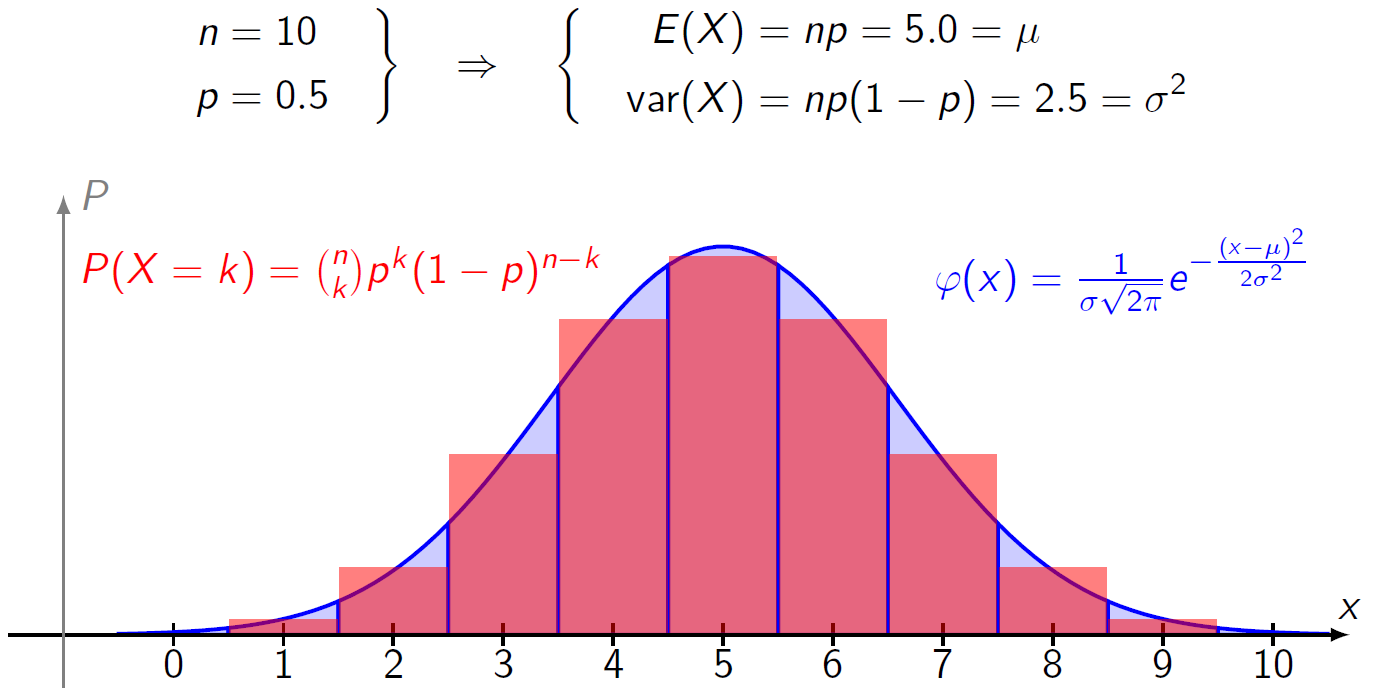
\includegraphics[width=0.75\columnwidth]{images/binomialverteilung_normalverteilung.png}
\end{center}

\subsection{Approximation für \textbf{seltene} Ereignisse (Poisson)}

\textbf{Voraussetzung:} Grenzwert $n \to \infty$ mit $n \cdot p = \lambda = $ erwartete Anzahl Ereignisse konstant (d.h. $p \to 0$) \\
\textbf{Wenn an der Prüfung \crd{SELTEN} in der Aufgabenstellung steht!!}

$$ \boxed{ P(X = k) = \begin{pmatrix} n \\ k \end{pmatrix} p^k (1-p)^{n-k} = e^{- \lambda} \frac{\lambda^k}{k!} = P_{\lambda}(k) } $$

Parameter: $\lambda = n \cdot p$ \quad (erwartete \# Ereignisse im Intervall $x$)

\vspace{0.2cm}

Summe von Wahrscheinlichkeiten, z.B. $P(k \leq 3)$: siehe Abschnitt \ref{sec:poisson-eigenschaften}


\subsection{Hypergeometrische Verteilung}

\textbf{Voraussetzung:} Von $N$ Objekten sind $M$ markiert. Daraus werden $n$ Objekte zufällig ausgewählt.


\subsubsection{Hypergeometrische Verteilung}

$X = $ Anzahl markierte Objekte unter den zufällig ausgewählten $n$ Objekten \\
Die Wahrscheinlichkeit, dass \textbf{genau $\boldsymbol{m}$ markierte Objekte gezogen} werden lautet:
$$ \boxed{ P(X = m) = \frac{ \begin{pmatrix} M \\ m \end{pmatrix} \begin{pmatrix} N-M \\ n-m \end{pmatrix} }{\begin{pmatrix} N \\ n \end{pmatrix}} } $$
\textbf{Notation: } $X \sim \mathrm{H}(N, M, n) $


\subsubsection{Eigenschaften der Hypergeometrischen Verteilung}

\myul{\textbf{Erwartungswert $\bm{E(X)}$ und Varianz $\bm{\var(X)}$}}

\begin{minipage}[c]{0.3\columnwidth}
	$$ \boxed{ E(X) = n \, \frac{M}{N} } $$
\end{minipage}
\hfill
\begin{minipage}[c]{0.66\columnwidth}
	$$ \boxed{ \var(X) = n \, \frac{M}{N} \Big( 1 - \frac{M}{N} \Big) \frac{N-n}{N-1} } $$
\end{minipage}


\example{Hypergeometrische Verteilung}

In einer Kiste mit 20 Äpfeln sind 5 wurmstichig. \\
Wie gross ist die Wahrscheinlichkeit, in einer Stichprobe von 8 Äpfel 2 wurmstichtige zu finden? \\
$N = 20$, $M = 5$, $n = 8$, $m = 2$

$$ P(X = 2) = \frac{ \begin{pmatrix} 5 \\ 2 \end{pmatrix} \begin{pmatrix} 15 \\ 6 \end{pmatrix} }{\begin{pmatrix} 20 \\ 8 \end{pmatrix}} = 0.3973 $$


\subsubsection{Begründung Hypergeometrische Verteilung}

\begin{minipage}{0.4\columnwidth}
	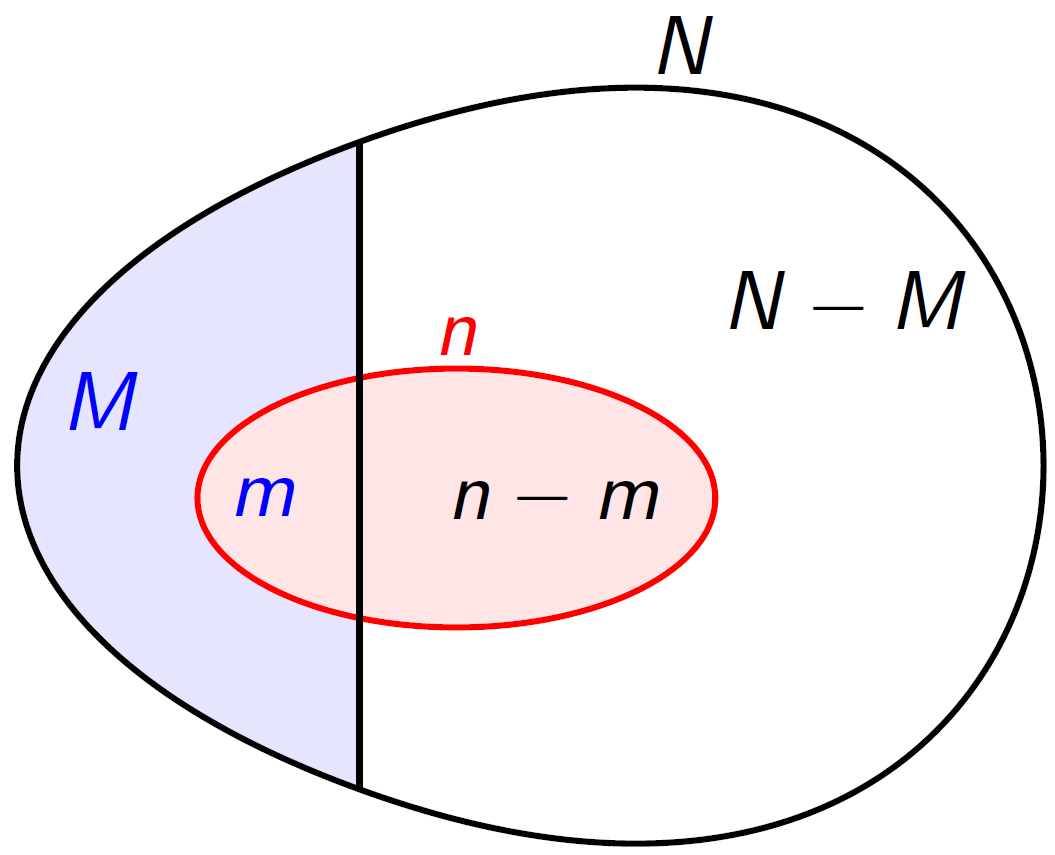
\includegraphics[width=\columnwidth]{images/begruendung_hypergeometrische_verteilung_1.png}
\end{minipage}
\hfill
\begin{minipage}{0.4\columnwidth}
	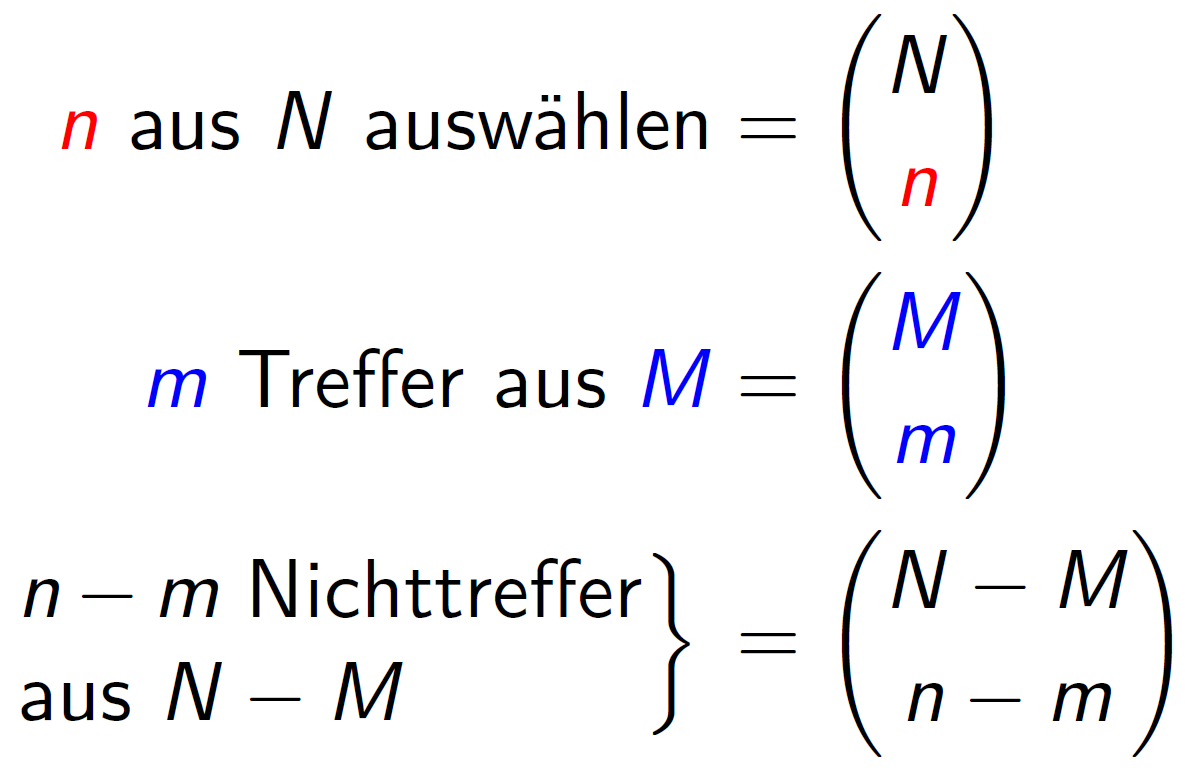
\includegraphics[width=\columnwidth]{images/begruendung_hypergeometrische_verteilung_2.png}
\end{minipage}


\subsection{Potenzverteilung (Skaleninvariante Prozesse)}

\subsubsection{Skaleninvarianz}

Ein Prozess ist \textbf{skaleninvariant}, wenn er auf jeder Skala \textbf{gleich} abläuft.

\vspace{0.2cm}

Skaliere $x$ mit $b$ \textrightarrow\ Form von $\varphi(x)$ ändert sich nicht

$$ \varphi(bx) = g(b) \, \varphi(x) \quad \text{für } x > x_{\rm min} $$
Faktor $g(b):$ Renormierung


\subsubsection{Potenzverteilung}

\vspace{-0.2cm}

$$ \boxed{ \varphi(x) = C \, e^{- \alpha} \quad \text{mit } \alpha = -g'(1) }$$
Beschränke auf $x > x_{\rm min}$ und wähle $C$ für korrekte Normierung

\vspace{0.2cm}

\begin{minipage}{0.55\columnwidth}
	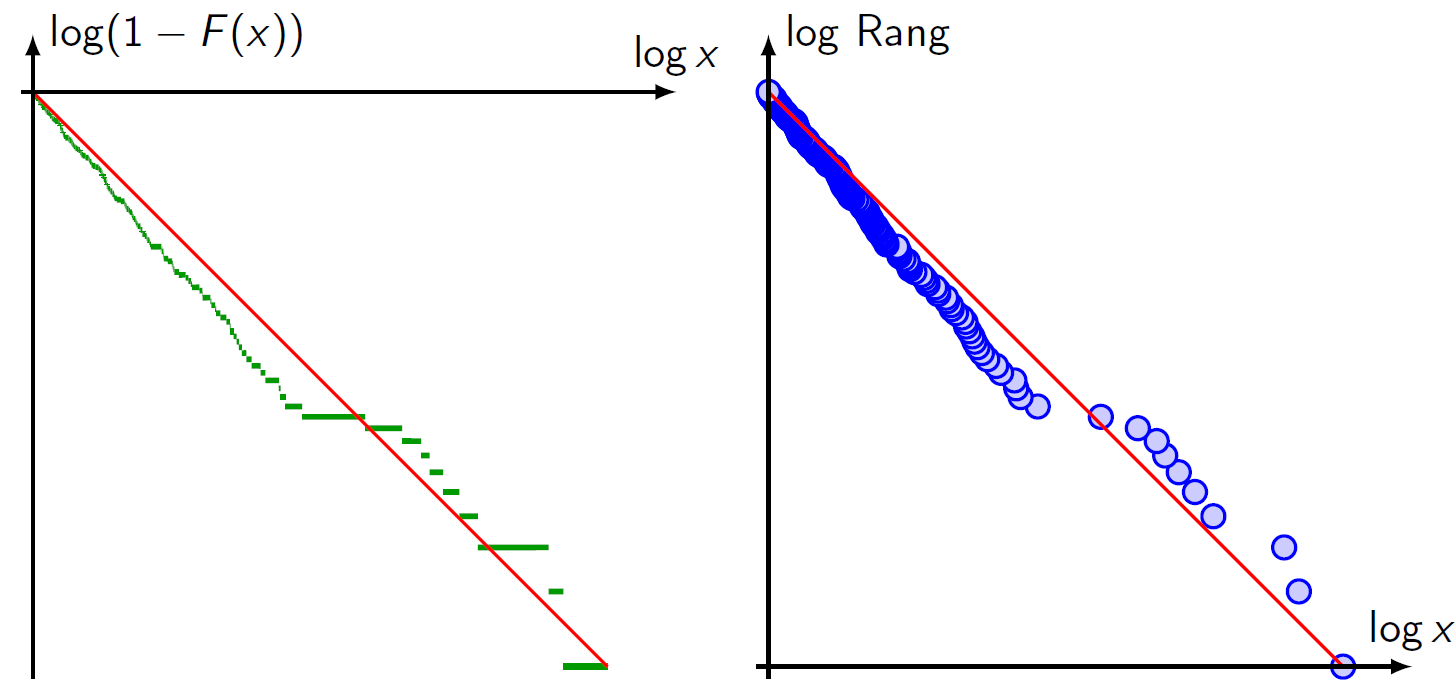
\includegraphics[width=\columnwidth]{images/potenzverteilung.png}
\end{minipage}
\hfill
\begin{minipage}{0.38\columnwidth}
	Geradengleichung in \\
	log-log-Skala
	$$ \log(\varphi(x)) = g'(1) \cdot \log(x) + c $$
\end{minipage}


\subsubsection{Anwendungen}

\begin{minipage}[t]{0.48\columnwidth}
	\begin{itemize}
		\item Städte und Bewohner
		\item Tierarten und ihre Häufigkeit
		\item Mondkrater und Durchmesser
		\item Bücher und Bestseller
	\end{itemize}
\end{minipage}
\hfill
\begin{minipage}[t]{0.48\columnwidth}
	\begin{itemize}
		\item Namen und Häufigkeit
		\item Einkommensverteilung
		\item Skaleninvariante Prozesse
	\end{itemize}
\end{minipage}


\subsubsection{Potenzgesetze für skaleninvariante Prozesse}

\myul{\textbf{Wahrscheinlichkeitsdichte $\bm{\varphi(x)}$}}
$$ \varphi(x) = \begin{cases}
0 																			& x < x_{\rm min} 	\\
\frac{\alpha - 1}{x_{\rm min}} \Big( \frac{x}{x_{\rm min}} \Big)^{-\alpha} 	& x \geq x_{\rm min} 
\end{cases}$$ 


\myul{\textbf{Verteilungsfunktion $\bm{F(x)}$}}

$$ F(x) =  \begin{cases}
0 													& x < x_{\rm min} 		\\
1 - \Big( \frac{x}{x_{\rm min}} \Big)^{1 - \alpha} 	& x \geq x_{\rm min} 
\end{cases}$$ 

\vspace{0.2cm}

\renewcommand{\arraystretch}{1.4}
\begin{tabular}{lll}
	Median 			& $ \mathrm{med}(x) = 2^{\frac{1}{\alpha-1}} \, x_{\rm min} $ 	& für $\alpha > 1$ \\
	Erwartungswert 	& $E(X) = \frac{\alpha - 1}{\alpha - 2} \, x_{\rm min}$ 		& für $\alpha > 2$ \\
	Varianz 		& $ \var(X) = \Big( \frac{\alpha - 1}{\alpha - 3} - \Big( \frac{\alpha - 1}{\alpha - 2} \Big)^2 \Big) \, x_{\rm min}^2 $ & für $\alpha > 3$
\end{tabular}
\renewcommand{\arraystretch}{1}


\subsubsection{'80 / 20 Regel'}

\vspace{-0.4cm}

\begin{minipage}[t]{0.48\columnwidth}
	\begin{align*}
		P(x) 	&= \text{Anteil der Werte } \crd{>} \, x 			\\
				&= 1 - P(X \leq x) = 1 - F(x) 						\\
				&= \int\limits_x^{\infty} \varphi(\xi) \, \diff \xi 
	\end{align*}
\end{minipage}
\hfill
\begin{minipage}[t]{0.48\columnwidth}
	\begin{align*}
		W(x) 	&= \text{Anteil am kumulierten Wert} 									\\
				&= \frac{\int\limits_x^{\infty} \xi \, \varphi(\xi) \, \diff \xi}{E(X)} 
	\end{align*}
	$$ W(x)= P(x)^{\frac{\alpha-2}{\alpha-1}} = P(x)^{\lambda} $$ 
\end{minipage}

\vspace{0.2cm}

\begin{minipage}{0.48\columnwidth}
	$$ \boxed{ \alpha = \frac{\lambda - 2}{\lambda - 1} } $$
\end{minipage}
\hfill
\begin{minipage}{0.48\columnwidth}
	$$ \boxed{ \lambda = \frac{\log(W)}{\log(P)} } $$
\end{minipage}


\subsection{Gleichverteilung}

\begin{minipage}{0.48\columnwidth}
	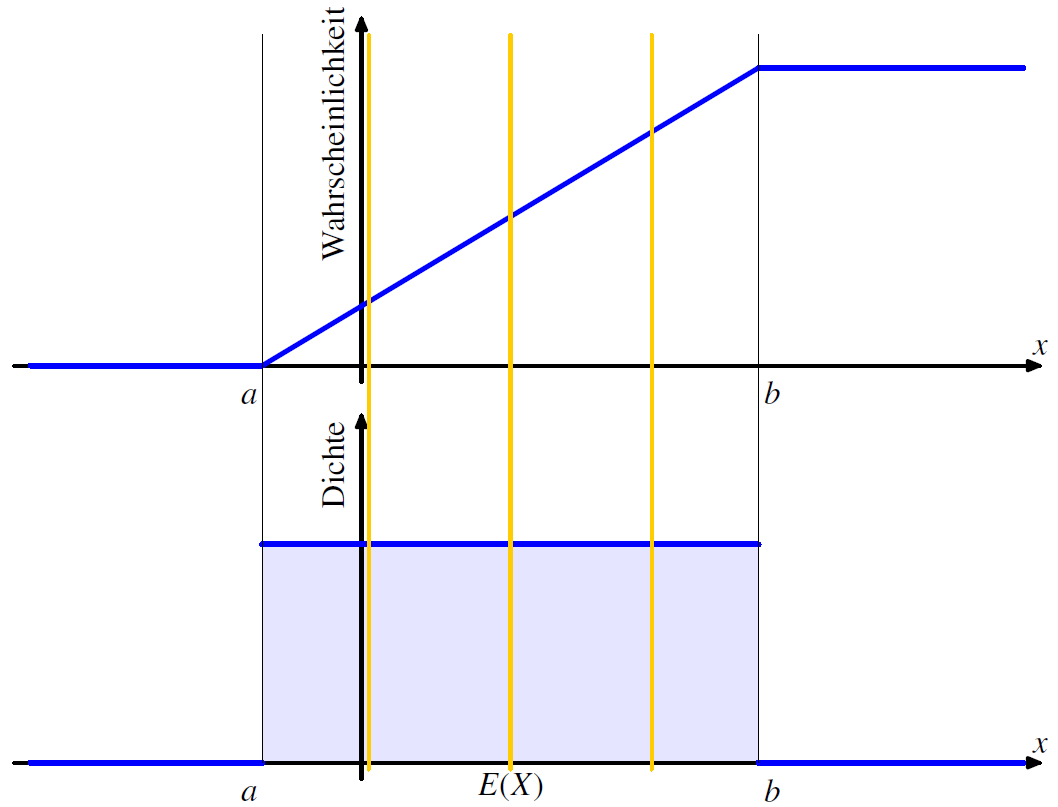
\includegraphics[width=\columnwidth]{images/gleichverteilung.png}
\end{minipage}
\hfill
\begin{minipage}{0.48\columnwidth}
	$\cgn{F(x)} =
	\begin{cases} 
	0 				& x \leq a 			\\
	\frac{x-a}{b-a} & a \leq x \leq b 	\\
	1 				& x > b 
	\end{cases}$ 
	
	\vspace{0.3cm}
	
	$\crd{\varphi(x)} = 
	\begin{cases} 
	\frac{1}{b-a} 	& a \leq x \leq b \\
	0 				& \text{sonst}
	\end{cases}$
\end{minipage}


\subsubsection{Eigenschaften der Gleichverteilung}

\myul{\textbf{Erwartungswert $\bm{E(X)}$ und Varianz $\bm{\var(X)}$}}

\begin{minipage}[c]{0.4\columnwidth}
	$$ \boxed{ E(X) = \frac{a + b}{2} } $$
\end{minipage}
\hfill
\begin{minipage}[c]{0.56\columnwidth}
	$$ \boxed{ \var(X) = \frac{(b - a)^2}{12} } $$
\end{minipage}


\vspace{0.15cm}
\textbf{Anwendungen:} Verteilung von Zufallszahlen, keine bevorzugten Werte

\columnbreak

